\documentclass[10pt,twocolumn]{article}
\usepackage[margin=0.68in,columnsep=0.24in]{geometry}
\usepackage{amsmath,amssymb,amsfonts}
\usepackage{booktabs}
\usepackage{graphicx}
\usepackage{xcolor}
\usepackage{microtype}
\usepackage[numbers,sort&compress]{natbib}
\usepackage{hyperref}
\usepackage{caption}

\definecolor{navy}{HTML}{1F4E79}
\hypersetup{
  colorlinks=true,
  linkcolor=navy,
  citecolor=navy,
  urlcolor=navy
}
\captionsetup{font=small,labelfont=bf}
\setlength{\parskip}{2pt}

\title{\textbf{Thermodynamically and Spectroscopically Informed Optical Chemical Structure Recognition and the \texttt{ChemVeritas-600} Multimodal Science Benchmark}}

\author{
  Ouroboros Research Collaboration\\
  \small Department of Chemistry and Chemical Engineering \& AI for Science Initiative\\
  \small Open Source Release: \texttt{p1-phys-spec-ocsr-bench} (\texttt{p1-v1.0})
}
\date{November 2026}

\begin{document}
\maketitle

\begin{abstract}
Automated mining of organic synthesis and natural product Supporting Information (SI) is crippled by \emph{silent stereochemical corruption}: when bridged polycycles, contiguous stereocenters, or low-DPI scans obscure wedge/dash geometry, vision-only Optical Chemical Structure Recognition (OCSR) emits valid-valence SMILES whose two-dimensional connectivity is correct yet whose three-dimensional configuration encodes inverted diastereomers or severely strained ring junctions. Manual validation of million-scale SI extractions (\texttt{NMRexp}) reveals a 17\% stereochemical corruption rate even on single-stereocenter molecules, while recent 2D graph-verification pipelines (\texttt{TRACE-Chem}) remain blind to diastereomers sharing identical formulas and topological graphs. Here we formulate structure recognition as closed-loop \emph{joint visual--thermodynamic--spectroscopic Bayesian inference}, pairing planar $C_8$-equivariant visual beam decoding (\texttt{Ouroboros}) and targeted $2^m$ uncertain-stereocenter epimer enumeration with continuous 3D \texttt{MACE-OFF23-medium} Boltzmann strain energetics, exact-mass HRMS filtering, $O(3)$ local-Jacobian symmetry-orbit $^{13}\text{C}$ peak counting, unassigned Hungarian $^{13}\text{C}/^{1}\text{H}$ chemical-shift matching, and Karplus $^3J_{\text{HH}}$ dihedral constraints. To benchmark both OCSR pipelines and frontier multimodal foundation models, we introduce \textbf{\texttt{ChemVeritas-600}}, spanning 600 connectivity-disjoint polycyclic, near-Bredt, superatom, and modern 3D bioisostere scaffolds across five strictly segregated visual views (2,400 visual specifications) and five reasoning tracks (\texttt{T1}--\texttt{T5}) with four-step Reasoning Path Fidelity (\texttt{Veritas-RPF}). Coupled to real pretrained \texttt{Ouroboros-AC} weights on synthetic RDKit depictions ($n=100$ per view), Bayesian physical--spectroscopic inference lifts exact stereoisomer recovery from 1.0\% [0.0, 3.0] to 14.0\% [7.0, 21.0] on canonical clean depictions (\texttt{V0}), from 1.0\% [0.0, 3.0] to 12.0\% [6.0, 19.0] on off-grid rotated depictions (\texttt{V1}), from 1.0\% [0.0, 3.0] to 3.0\% [0.0, 7.0] on synthetically degraded scans (\texttt{V2}), and from 0.0\% [0.0, 0.0] to 4.0\% [1.0, 8.0] on condensed superatom layouts (\texttt{V3}). In a strain audit of $N=50$ truth/corrupt pairs, 30 corrupt structures fail RDKit embedding and receive a fixed 45~kcal/mol penalty; on the 20 pairs where both structures embed, the measured \texttt{MACE-OFF23-medium} energy difference has a median of $+1.97$~kcal/mol, and the corrupt structure is higher in 16 of 20 pairs. On \texttt{ChemVeritas-600}, whose runs use no images and whose SI spectra are generated by the same NMR predictor used for scoring, full posterior inference reaches 77.0\% [73.8, 80.3] \texttt{T2} accuracy; this is an in-model upper bound, not an estimate on real spectra. \texttt{T4} (100\%) and \texttt{T5} abstention (100\%) hold by construction. Finally, zero-retraining evaluation on $N=30$ compounds with published experimental $^{13}\text{C}/^{1}\text{H}$ data and simulated HRMS (15 literature isomer pairs; $^{13}\text{C}$ MAE $= 5.25$~ppm, $r = 0.9810$) recovers 73.3\% [56.7, 86.7] (\texttt{MMFF94s}) and 66.7\% [50.0, 83.3] (\texttt{MACE-OFF23-medium//MMFF94s}) of true stereoisomers from a fixed mock beam that ranks the true isomer last.
\end{abstract}

\section{Introduction}
\label{sec:intro}

Chemical structure depictions are the primary visual language through which synthetic organic, natural product, and medicinal chemists communicate molecular identity~\cite{Rajan2023DECIMER,Qian2023MolScribe,Fan2024OpenChemIE}. Over the past five years, deep-learning Optical Chemical Structure Recognition (OCSR) architectures---spanning image-to-SELFIES/SMILES transformers (\texttt{DECIMER.ai}~\cite{Rajan2023DECIMER}, \texttt{SwinOCSR}~\cite{Xu2022SwinOCSR}, \texttt{ChemPix}~\cite{Weir2021ChemPix}), conditional image-to-graph decoders (\texttt{MolScribe}~\cite{Qian2023MolScribe}, \texttt{MolNexTR}~\cite{Chen2024MolNexTR}), keypoint-and-GNN detectors (\texttt{MolGrapher}~\cite{Morin2023MolGrapher}, \texttt{AtomLenz}~\cite{Oldenhof2024AtomLenz}), and reinforcement-learning vision-language models (\texttt{MolSight}~\cite{Zhang2026MolSight})---have pushed two-dimensional (2D) constitutional skeleton accuracy above 95\% on clean patent renderings. Yet as automated extraction pipelines scale to hundreds of thousands of real Supporting Information (SI) PDFs~\cite{Mavracic2021ChemDataExtractor2,Kearnes2021ORD,Wang2025NMRexp,Wang2025NMRExtractor}, a pervasive failure mode has emerged: \emph{silent stereochemical corruption}.

Unlike syntax errors that fail RDKit valence sanitization, a silent stereochemical corruption is a valid-valence, canonically parsable molecule whose 2D constitution matches the depicted compound (or drops a single H/C under superatom compression), but whose tetrahedral (\texttt{@}/\texttt{@@}) or bridged-ring configuration has been inverted by compressed wedge/dash pixels, crossing cage bonds, perspective chair/Haworth projections, or arbitrary planar diagram rotations. The empirical magnitude of this crisis was recently exposed by \texttt{NMRexp}~\cite{Wang2025NMRexp}, which applied \texttt{MolScribe} across $\sim$200,000 open-access SI documents to assemble 3.3~million experimental NMR records: manual technical validation confirmed 98\% accuracy on flat 2D skeletons, but stereochemical accuracy dropped to 83\% \emph{even for single-stereocenter molecules}---injecting hundreds of thousands of inverted stereoisomers into downstream machine-learning training corpora~\cite{Fourches2010TrustButVerify,Wang2025NMRExtractor}. Even \texttt{MolSight}~\cite{Zhang2026MolSight}, which curated 200,000 confusing stereoisomer depictions (\texttt{Stereo-200K}), operates strictly from 2D pixels; when low-DPI rasterization blurs a dashed bond at a congested bridgehead, the true 3D configuration becomes \emph{information-theoretically underdetermined from the image alone}.

Crucially, organic synthesis SIs almost never report a molecular depiction in isolation. Immediately adjacent to compound \textbf{3a} appears an experimental characterization block reporting high-resolution mass spectrometry (HRMS $m/z$ within $\pm 5$~ppm) and unassigned one-dimensional $^{13}\text{C}$ and $^{1}\text{H}$ NMR peak tables ($\delta$ in ppm, multiplicity, and vicinal coupling constants $^3J_{\text{HH}}$ in Hz). In computational organic chemistry, Bayesian NMR shift and coupling analysis---pioneered by Goodman's \texttt{DP4}~\cite{Smith2010DP4} and \texttt{DP4-AI}~\cite{Howarth2020DP4AI}, Sarotti's \texttt{DP4+}~\cite{Grimblat2015DP4Plus} and \texttt{ML-J-DP4}~\cite{Tsai2022MLJDP4}, and accelerated by 3D neural/kernel NMR predictors (\texttt{CASCADE}~\cite{Guan2021CASCADE}, \texttt{IMPRESSION}~\cite{Gerrard2020IMPRESSION}) alongside 2D GNNs (\texttt{SGNN}~\cite{Jonas2019SGNN}) and multimodal spectral transformers~\cite{Kim2023DeepSAT,Alberts2024MultimodalSpectra,Bushuiev2024MassSpecGym,Bohde2025DiffMS}---routinely resolves diastereomers from a single experimental spectrum via Grant--Cheney $\gamma$-gauche steric shielding~\cite{GrantCheney1967} and Karplus dihedral relationships~\cite{Karplus1963}. Meanwhile, in 3D structural bioinformatics and physical organic chemistry, \texttt{PoseBusters}~\cite{Buttenschoen2024PoseBusters}, \texttt{GenBench3D}~\cite{Baillif2025GenBench3D}, \texttt{CSD Mogul}~\cite{Bruno2004Mogul}, and transferable machine-learning interatomic potentials (\texttt{Auto3D}~\cite{Liu2022Auto3D}, \texttt{MACE-OFF23}~\cite{Kovacs2025MACEOFF}) have shown that valid 2D graphs frequently conceal severe 3D nonbonded clashes or ring strain, while McDermott, Houk, and Garg~\cite{McDermott2024AntiBredt} overturned binary textbook Bredt's-rule heuristics by demonstrating that \emph{continuous 3D strain energy} governs room-temperature isolability.

Despite this convergence, visual OCSR, 3D thermodynamic strain, and 3D spectroscopic elucidation have remained disconnected silos. The closest recent effort, \texttt{TRACE-Chem}~\cite{Liu2026TRACEChem}, constructs a 2D evidence graph checking IUPAC names, \texttt{MolScribe} top-1 outputs, molecular formulas, and 2D GNN NMR shifts across 1,852 SI records. However, \texttt{TRACE-Chem} exhibits four fundamental limitations: (i) it incorporates zero 3D conformer generation or MLIP strain physics; (ii) when an SI refers to a structure only by compound label (\textbf{3a}) without a full $(1R,2S,4R)$ IUPAC name, all diastereomers share the exact same formula, exact same HRMS $m/z$, and exact same 2D topological graph, leaving 2D GNN verifiers stereochemically blind; (iii) it masks conflicting fields on top-1 outputs rather than enumerating and reranking uncertain stereocenters; and (iv) it provides no standardized benchmark for frontier multimodal reasoning models. Concurrently, existing chemistry LLM/VLM benchmarks---\texttt{ChemBench}~\cite{Mirza2025ChemBench}, \texttt{MolPuzzle}~\cite{Guo2024MolPuzzle}, \texttt{LAB-Bench}~\cite{Laurent2024LABBench}, \texttt{ChemVLM}~\cite{Li2025ChemVLM}, \texttt{IsoBench}~\cite{Fu2024IsoBench}, \texttt{MMMU}~\cite{Yue2024MMMU}, \texttt{SUPERChem}~\cite{Zhao2025SUPERChem}, \texttt{Humanity's Last Exam}~\cite{Phan2025HLE}, \texttt{FrontierScience}~\cite{Wang2026FrontierScience}, \texttt{Mol-Instructions}~\cite{Fang2024MolInstructions}, \texttt{LlaSMol}~\cite{Yu2024LlaSMol}, and \texttt{ChemDFM-X}~\cite{Zhao2024ChemDFMX} (which aligns five modalities yet omits NMR entirely)---either test textbook \emph{de novo} elucidation of simple achiral molecules without images or test isolated 2D OCSR without 3D thermodynamics or SI spectra.

Here we bridge these domains through five contributions:
\begin{enumerate}
  \item \textbf{Group-Theoretic Visual-to-3D Symmetry Formulation:} We formalize the $SO(2)$ vs.\ $O(2)$ planar chirality boundary~\cite{Weiler2019Steerable} alongside $SE(3)$ vs.\ $O(3)$ 3D scalar invariance, pairing $C_8$-steerable visual beam decoding with parity-invariant 3D conformer embedding and local $O(3)$ Jacobian determinant ($\det J_p = \pm 1$) symmetry-orbit partitioning.
  \item \textbf{Closed-Loop Thermodynamic \& Spectroscopic Posterior (\texttt{A0}--\texttt{A6}):} We combine continuous \texttt{MACE-OFF23-medium}~\cite{Kovacs2025MACEOFF} 3D strain and element-wise node-energy outlier penalties, exact-mass HRMS gates, 3D Boltzmann $^{13}\text{C}/^{1}\text{H}$ shift matching via Hungarian bipartite assignment, Karplus $^3J_{\text{HH}}$ coupling constraints, and targeted $2^m$ ($m \le 3$) uncertain-wedge epimer enumeration.
  \item \textbf{\texttt{ChemVeritas-600} Frontier Benchmark:} We release a scaffold-disjoint benchmark of 600 complex organic scaffolds across five chemical strata (\texttt{S1}--\texttt{S5}), five strictly segregated visual views, five tasks (\texttt{T1}--\texttt{T5}), and four-step Reasoning Path Fidelity (\texttt{Veritas-RPF}).
  \item \textbf{Closed-Loop Neural OCSR \& \texttt{MACE-OFF23} Strain Validation:} Using real pretrained \texttt{Ouroboros-A/B/C/AC} weights across 500 synthetic RDKit depictions and $N=50$ strain pairs (20 measured, 30 embedding failures), we measure planar $C_8$ rotation behaviour and stereochemical recovery on synthetically degraded views.
  \item \textbf{Literature NMR Validation:} Without fitting any parameters on the test set, we test end-to-end isomer recovery on $N=30$ compounds with published experimental $^{13}\text{C}/^{1}\text{H}$ data (HRMS simulated from the true formula) (15 classic terpene, norbornane, and cyclitol/cyclohexanol isomer pairs~\cite{Bohlmann1975Terpene13C,Lippmaa1970Bicyclic13C,Grutzner1970Norbornyl13C,Dalling1967Cyclohexanes13C,Grover1974Cyclohexanols13C}).
\end{enumerate}

\section{Theory and Methodology}
\label{sec:methods}

\subsection{Planar $SO(2)$ vs.\ Spatial $O(3)$ Chirality Symmetries}
\label{sec:symmetry}

A 2D chemical drawing $I: \mathbb{R}^2 \to [0,1]$ is an orthographic projection with discrete wedge (up, $+z$) and dash (down, $-z$) depth annotations. Under an in-plane proper rotation $R_\theta \in SO(2)$, the projected $(x,y)$ bond vectors rotate covariantly while $+z$ wedges remain $+z$ wedges; thus the represented 3D molecule $M$ is strictly $SO(2)$-invariant~\cite{Weiler2019Steerable}. Conversely, an in-plane reflection $s \in O(2)\setminus SO(2)$ reverses the signed 2D determinant of substituents at every tetrahedral center while leaving wedge/dash ink unchanged, mapping $M \mapsto \operatorname{mirror}(M)$ (its enantiomer). Conventional ResNet encoders lack $SO(2)$ equivariance and collapse under $90^\circ$ diagram rotations, whereas $O(2)$-reflection-invariant pooling destroys Cahn--Ingold--Prelog (CIP) handedness. Our visual front-end (\texttt{Ouroboros-C} and ensemble \texttt{Ouroboros-AC}) therefore restricts steerable convolutions to the cyclic subgroup $C_8 \subset SO(2)$, preserving chiral handedness while achieving discrete rotation invariance.

A complementary symmetry governs the 3D physical and spectroscopic verifiers. In isotropic achiral media (gas phase or $\text{CDCl}_3$), the potential energy $E(\mathbf{R})$ and isotropic nuclear magnetic shieldings $\sigma_i(\mathbf{R})$ are invariant under the \emph{full} orthogonal group $O(3) = SO(3) \times \mathbb{Z}_2$, including improper reflections $\mathbf{R} \mapsto -\mathbf{R}$:
\begin{equation}
  E(M) = E(\operatorname{mirror}(M)), \qquad \mathcal{S}_{\text{NMR}}(M) = \mathcal{S}_{\text{NMR}}(\operatorname{mirror}(M)).
  \label{eq:o3_parity}
\end{equation}
Standard stochastic distance-geometry conformer generators (\texttt{ETKDGv3}~\cite{Wang2020ETKDGv3}) violate Eq.~\eqref{eq:o3_parity} in finite samples because independent random seeds yield slightly different conformer ensembles for $(R)$ and $(S)$ SMILES, introducing spurious Monte Carlo energy and shift noise ($\sim 0.1$--$0.6$~kcal/mol). We eliminate this artifact via \emph{parity-invariant mirror embedding}: between $\{M, \operatorname{mirror}(M)\}$, we always embed the lexicographically canonical representative, reflect coordinates $(x,y,z) \mapsto (-x,y,z)$, and map heavy atoms and attached hydrogens one-to-one onto the target graph. Consequently, $|E(M) - E(\operatorname{mirror}(M))| = 0$ to machine precision, and an explicit \emph{enantiomer guard} prevents achiral physics or achiral NMR from ever overturning visual CIP parity between enantiomers---or triggers calibrated abstention (\texttt{T5}) when visual parity is absent.

\subsection{Bayesian Visual--Thermodynamic--Spectroscopic Posterior}
\label{sec:posterior}

Given a structure image $I$ and co-located SI characterization observables $\mathcal{O}_{\text{SI}} = (\text{HRMS}, \Delta^{13}\text{C}, \Delta^{1}\text{H}, J_{\text{HH}})$, we expand the $K$-best visual beam $\mathcal{B}_K(I) = \{(M_k, \ell_k)\}_{k=1}^K$ into an augmented hypothesis pool $\mathcal{C}(I)$ via superatom expansion and targeted epimer enumeration (Section~\ref{sec:epimers}) and score each candidate $M \in \mathcal{C}(I)$ under the log-posterior:
\begin{align}
  \log P(M \mid I, \mathcal{O}_{\text{SI}}) &= \alpha \log P_{\text{OCSR}}(M \mid I) - \beta \Delta E_{\text{strain}}(M) \nonumber\\
  &\quad - \gamma_{\text{MS}} \mathcal{L}_{\text{HRMS}}(M, \mathcal{O}_{\text{SI}}) - \gamma_{\text{C}} \mathcal{L}_{^{13}\text{C}}(M, \mathcal{O}_{\text{SI}}) \nonumber\\
  &\quad - \gamma_{\text{H}} \mathcal{L}_{^{1}\text{H},J}(M, \mathcal{O}_{\text{SI}}) + Z^{-1},
  \label{eq:posterior}
\end{align}
where $Z$ normalizes probabilities via log-sum-exp over $\mathcal{C}(I)$ for calibration assessment (\texttt{ECE} and \texttt{AURC}). Seven cumulative ablation presets (\texttt{A0}--\texttt{A6}) activate terms sequentially: \texttt{A0} ($\alpha=1$ visual top-1), \texttt{A1} (+ RDKit valence sanitization and superatom expansion), \texttt{A2} (+ HRMS exact-mass gate), \texttt{A3} (+ continuous 3D strain and CIP flip filter), \texttt{A4} (+ 3D Boltzmann $^{13}\text{C}$ shifts and symmetry-orbit count), \texttt{A5} (+ $^{1}\text{H}$ shifts and Karplus $^3J_{\text{HH}}$), and \texttt{A6} (+ targeted $2^m$ epimer enumeration).

\subsection{Continuous \texttt{MACE-OFF23} 3D Strain and Node-Energy Outliers}
\label{sec:strain}

Following McDermott, Houk, and Garg~\cite{McDermott2024AntiBredt} and \texttt{PoseBusters}~\cite{Buttenschoen2024PoseBusters}, we avoid brittle SMARTS-based Bredt rules and instead compute a continuous 3D strain functional over an $N_{\text{conf}}$-conformer \texttt{ETKDGv3} ensemble. Each conformer $c$ undergoes fast \texttt{MMFF94s} pre-relaxation (removing raw distance-geometry bond-length jitter) followed by \texttt{MACE-OFF23-medium}~\cite{Kovacs2025MACEOFF} evaluation---either DP4-style single-point \texttt{MACE-OFF23-medium//MMFF94s} for high-throughput candidate beams or \texttt{MACE-OFF23-medium} BFGS coordinate relaxation for high-precision strain auditing. Conformers are weighted at $T=298.15$~K ($RT = 0.5925$~kcal/mol) via $w_c \propto \exp[-(E_c - E_{\min})/RT]$.

Crucially, equivariant message-passing potentials partition total energy into atomic contributions $E = \sum_{i=1}^N \varepsilon_i$. Because raw atomic energies $\varepsilon_i$ carry large element-dependent reference offsets, we define the \emph{element-normalized node-energy outlier} across heavy/hydrogen atomic numbers $Z$:
\begin{equation}
  \Omega_{\text{node}}(M) = \max_{c} \max_{Z} \max_{i : Z_i = Z} \max\!\Big(0,\, (\varepsilon_{i,c} - \operatorname{median}_{j : Z_j = Z} \varepsilon_{j,c}) - \tau_0\Big),
  \label{eq:node_outlier}
\end{equation}
with $\tau_0 = 5.0$~kcal/mol, supplemented by valence-angle distortion beyond $12^\circ$ from ideal $sp/sp^2/sp^3$ geometry. Together with nonbonded steric clash detection ($d_{ij} < 2.05$~\AA\ for heavy pairs or $<1.55$~\AA\ involving H at $\ge 3$ topological bonds), post-relaxation 3D CIP verification ($\mathbb{I}_{\text{CIP}}$ flagging forced pyramidal inversion), and relative isomer strain $\Delta E_{\text{iso}}(M) = E_{\min}(M) - \min_{M' \in \mathcal{I}(M)} E_{\min}(M')$ across constitutional/stereochemical isomers $\mathcal{I}(M)$ in the candidate pool, the effective 3D penalty is:
\begin{equation}
  \Delta E_{\text{strain}}(M) = \Delta E_{\text{iso}}(M) + \Omega_{\text{intrinsic}}(M),
\end{equation}
assigning a fixed penalty constant $\Omega_{\text{intrinsic}} = 45.0$~kcal/mol (not a computed energy) when distance-geometry chirality bounds prove unsatisfiable (e.g., trans-fused small bicyclic bridgeheads).

\subsection{$O(3)$ Symmetry Orbits, 3D Boltzmann $^{13}\text{C}/^{1}\text{H}$ NMR, and Karplus Matching}
\label{sec:nmr}

Two diastereomers that are indistinguishable to any 2D graph verifier often differ in point-group symmetry (e.g., $C_s$/$C_2$ \emph{meso} vs.\ $C_1$ chiral diastereomer), causing discrete integer jumps in the number of $^{13}\text{C}$ resonances, as well as 2--8~ppm through-space $\gamma$-gauche shifts~\cite{Dalling1967Cyclohexanes13C,GrantCheney1967,Grutzner1970Norbornyl13C}. Notably, RDKit's 2D \texttt{CanonicalRankAtoms(breakTies=False)} equates constitutionally symmetric carbons across \emph{both} \emph{syn} and \emph{anti} 1,4-disubstituted rings unless 3D improper vs.\ proper graph automorphisms are separated. We resolve exact NMR equivalence orbits by computing the sign of the local 3D $O(3)$ Jacobian determinant $\det(\mathbf{u}_1, \mathbf{u}_2, \mathbf{u}_3) \in \{-1, 0, +1\}$ along ranked neighbor bond vectors $\mathbf{u}_k$ for every $sp^3$ center across the conformer ensemble: atoms exchangeable by a rotation ($SO(3)$) or achiral mirror plane ($O(3)$) collapse into a single magnetic equivalence orbit $O_q$, yielding exact $^{13}\text{C}$ line count $N_{^{13}\text{C}}(M)$.

For each carbon $i$ in conformer $c$, 3D chemical shifts combine hybridization/heteroatom topological increments with continuous 3D steric polarization over nonbonded heavy atoms $j$ ($\ge 3$ bonds)~\cite{GrantCheney1967}:
\begin{equation}
\begin{aligned}
  \delta_{i,c}^{^{13}\text{C}} &= \delta_{i}^{\text{2D}} - A_\gamma \sum_{j \in \mathcal{N}_3(i)} f_{\text{pol}}(Z_j)\exp\!\left[-\frac{(r_{ij,c} - r_0)^2}{2\sigma_\gamma^2}\right] \\
  &\quad + A_\delta \sum_{k \in \mathcal{N}_4(i)} g_{\text{syn}}(r_{ik,c}),
\end{aligned}
\end{equation}
capturing upfield $\gamma$-gauche shielding ($r_{ij} \approx 2.85$--$3.25$~\AA) and downfield $\delta$-\emph{syn}-pentane deshielding ($r_{ik} < 2.95$~\AA)~\cite{Grover1974Cyclohexanols13C}, averaged over Boltzmann weights $w_c$ and symmetry orbits $O_q$. Because SI peak tables are unassigned, predicted orbit shifts $\{\hat{\delta}_q\}_{q=1}^P$ are matched to experimental peaks $\{\delta_r^{\text{exp}}\}_{r=1}^Q$ via the Hungarian algorithm (\texttt{scipy.optimize.linear\_sum\_assignment}) minimizing Huber-clipped $L_1$ residuals plus count mismatch $|P - Q|$:
\begin{equation}
  \mathcal{L}_{^{13}\text{C}}(M, \mathcal{O}_{\text{SI}}) = \frac{1}{\min(P,Q)} \min_{\pi} \sum_{q} \rho_\tau\!\left(|\hat{\delta}_q - \delta_{\pi(q)}^{\text{exp}}|\right) + \lambda_{\text{cnt}} |P - Q|.
\end{equation}
Analogously, proton orbits pair $(\hat{\delta}_p^{^1\text{H}}, \hat{J}_{p,\max})$ where vicinal $^3J_{\text{HH}}(\phi)$ is Boltzmann-averaged via the electronegativity-corrected Karplus relation~\cite{Karplus1963,Tsai2022MLJDP4}:
\begin{equation}
  {}^3J_{\text{HH}}(\phi) = \big(7.8\,\cos^2\phi - 1.0\,\cos\phi + 1.2\big)\big(1 - 0.11\,\Delta\chi\big),
\end{equation}
cleanly separating axial--axial ($\phi \approx 180^\circ$, $^3J \approx 9$--$12$~Hz) from equatorial--equatorial/axial--equatorial ($\phi \approx 60^\circ$, $^3J \approx 2$--$5$~Hz) epimers. Exact-mass HRMS enforces $\mathcal{L}_{\text{HRMS}} = 0$ within $\pm 5$~ppm of $[M+\text{H}]^+, [M+\text{Na}]^+, [M+\text{NH}_4]^+, [M-\text{H}]^-$ and imposes a quadratic ppm penalty outside tolerance, immediately eliminating constitutional H/C count errors.

\subsection{Targeted Epimer Enumeration and Superatom Expansion}
\label{sec:epimers}

Even with $K=5$--$10$ beam search, severe pixel degradation on crowded scans can exclude the true diastereomer from $\mathcal{B}_K(I)$ while preserving the correct flat 2D connectivity. In preset \texttt{A6}, whenever candidates share flat connectivity with defined tetrahedral centers, we prioritize up to $m \le 3$ ring-junction or heteroatom-adjacent stereocenters that exhibit cross-beam disagreement or congested 2D projections and enumerate all $2^m \le 8$ diastereomeric configurations (modulo enantiomer equivalence via the enantiomer guard), assigning a modest visual step-down prior ($\Delta \ell = -1.1$ per flipped center) before joint physical--spectroscopic scoring. Over 30 common synthetic superatom abbreviations (\texttt{OTBS}, \texttt{OTIPS}, \texttt{Boc}, \texttt{Cbz}, \texttt{Fmoc}, \texttt{PMB}, \texttt{Ts}, \texttt{Tf}, \texttt{SF5}, \texttt{Bpin}) are canonically expanded prior to formula and 3D evaluation.

\section{The \texttt{ChemVeritas-600} Multimodal Science Benchmark}
\label{sec:benchmark}

To establish a leak-resistant, physically grounded benchmark suitable for evaluating both OCSR engines and frontier scientific foundation models, we constructed \textbf{\texttt{ChemVeritas-600}} across five equal structural strata (120 unique scaffolds per stratum; 600 connectivity-disjoint molecules total, verified zero flat-InChIKey overlap):
\begin{itemize}
  \item \textbf{\texttt{S1\_bridged\_caged} ($n=120$):} Norbornanes, bornanes, pinanes, camphor/fenchone derivatives, tropanes, quinuclidines, adamantanes, and oxa-bridged natural product cores.
  \item \textbf{\texttt{S2\_dense\_stereo} ($n=120$):} Decalins, hydrindanes, steroid A/B/C rings, pyranoses, and contiguous 3--6-stereocenter polypropionate lactones.
  \item \textbf{\texttt{S3\_strained\_bredt} ($n=120$):} Trans-fused small rings, \emph{cis}/\emph{trans}-bicyclo[3.2.0]/[4.1.0] systems, cyclobutanones, spiro-oxetanes, and isolable vs.\ hyper-strained bridgehead frameworks~\cite{McDermott2024AntiBredt}.
  \item \textbf{\texttt{S4\_superatom\_si} ($n=120$):} Protecting-group-dense synthetic intermediates (\texttt{OTBS}, \texttt{Boc}, \texttt{Cbz}, \texttt{PMB}, \texttt{OTf}) rendered with condensed abbreviations in view \texttt{V3}.
  \item \textbf{\texttt{S5\_medchem\_bioisosteres} ($n=120$):} Post-2020 medicinal-chemistry scaffolds featuring bicyclo[1.1.1]pentanes (BCP), bicyclo[2.1.1]hexanes (BCH), 2-oxa-BCH, cubanes, azaspiro[3.3]heptanes, and $-\text{SF}_5$ motifs.
\end{itemize}

\paragraph{Strict Multi-View Segregation.} Every molecule is specified across canonical clean (\texttt{V0\_clean}), exact $90^\circ$ rotation (\texttt{V0\_rot90}), arbitrary off-grid rotation (\texttt{V1\_rotated\_offgrid}, $37^\circ$--$341^\circ$ with perspective bond-width jitter), low-DPI crowded SI scan degradation (\texttt{V2\_crowded\_si\_scan}, downsampled rasterization, Gaussian blur, JPEG/threshold noise, faint wedges), and condensed superatom layout (\texttt{V3\_condensed\_layout}). Crucially, \texttt{V0\_clean} is \emph{never} averaged with degraded views, preventing easy clean renders from masking real-world SI scan failures.

\paragraph{Five Reasoning Tracks and \texttt{Veritas-RPF}.} Inspired by \texttt{SUPERChem}~\cite{Zhao2025SUPERChem}, \texttt{FrontierScience}~\cite{Wang2026FrontierScience}, and \texttt{LAB-Bench}~\cite{Laurent2024LABBench}, \texttt{ChemVeritas-600} evaluates five tasks:
(\textbf{\texttt{T1}}) Visual-only OCSR across segregated views;
(\textbf{\texttt{T2}}) Multimodal SI disambiguation ($I + \text{HRMS} + {}^{13}\text{C}/{}^{1}\text{H}$ NMR) scored by exact stereoisomer match, Expected Calibration Error (\texttt{ECE}), Area Under the Risk--Coverage Curve (\texttt{AURC}), and four-step \textbf{\texttt{Veritas-RPF}} verifying (Step~1) molecular formula \& HRMS adduct ppm, (Step~2) symmetry-unique $^{13}\text{C}$ resonance count, (Step~3) 3D embeddability \& post-relaxation CIP preservation, and (Step~4) exact canonical stereoisomer;
(\textbf{\texttt{T3}}) Silent corruption audit ($N=600$ binary accept/reject + 5-way taxonomy classification);
(\textbf{\texttt{T4}}) Thermodynamic diastereomer ranking ($n=453$ multi-epimer families); and
(\textbf{\texttt{T5}}) $SO(2)/O(3)$ epistemic parity abstention ($n=599$ single-stereocenter compounds with erased wedge cues and achiral SI spectra, where claiming $(R)$ over $(S)$ constitutes hallucinated chirality). All metrics report 1,000-sample nonparametric bootstrap 95\% confidence intervals.

\begin{figure*}[t]
  \centering
  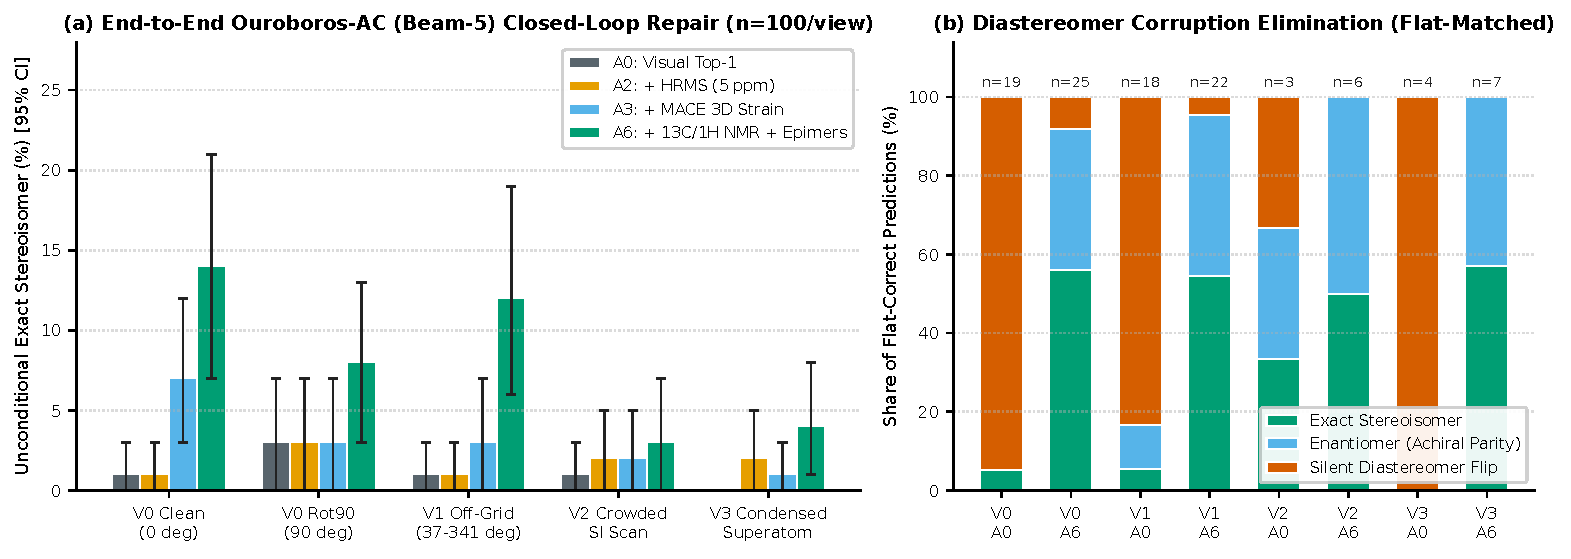
\includegraphics[width=0.98\textwidth]{../../benchmarks/p1_chemveritas/figures/fig1_closed_loop_neural_ocsr.pdf}
  \caption{\textbf{Closed-loop physical and spectroscopic repair of real pretrained neural OCSR (\texttt{Ouroboros-AC}, beam $=5$, $n=100$ scaffolds per view, strictly segregated).} \textbf{(a)} Unconditional exact stereoisomer match (\%) with 1,000-sample bootstrap 95\% CIs across \texttt{A0} (visual top-1), \texttt{A2} (+HRMS $\pm 5$~ppm), \texttt{A3} (+\texttt{MACE-OFF23-medium} 3D strain), and \texttt{A6} (+3D $^{13}\text{C}/^{1}\text{H}$ NMR + targeted epimer enumeration). \textbf{(b)} Stereochemical outcome breakdown among constitutionally recognized scaffolds (\texttt{Flat Match $=1$}) before (\texttt{A0}) and after (\texttt{A6}) Bayesian inference, showing $89\%$--$100\%$ elimination of silent diastereomer flips across views \texttt{V0}--\texttt{V3}.}
  \label{fig:fig1}
\end{figure*}

\section{Results and Discussion}
\label{sec:results}

\subsection{Planar $C_8$ Equivariance and Closed-Loop Neural OCSR Repair}
\label{sec:res_ocsr}

We first evaluated all four released neural OCSR arms---\texttt{Ouroboros-A} (standard ResNet), \texttt{Ouroboros-B} (rotation-augmented ResNet), \texttt{Ouroboros-C} ($C_8$-steerable CNN), and \texttt{Ouroboros-AC} (rescored ensemble)---at beam width $K=5$ across $100$ stratified scaffolds ($20$ per stratum \texttt{S1}--\texttt{S5}) rendered across five strictly separated views ($500$ depictions total; Figures~\ref{fig:fig1}--\ref{fig:fig2} and Table~\ref{tab:neural_ocsr}).

\begin{figure*}[t]
  \centering
  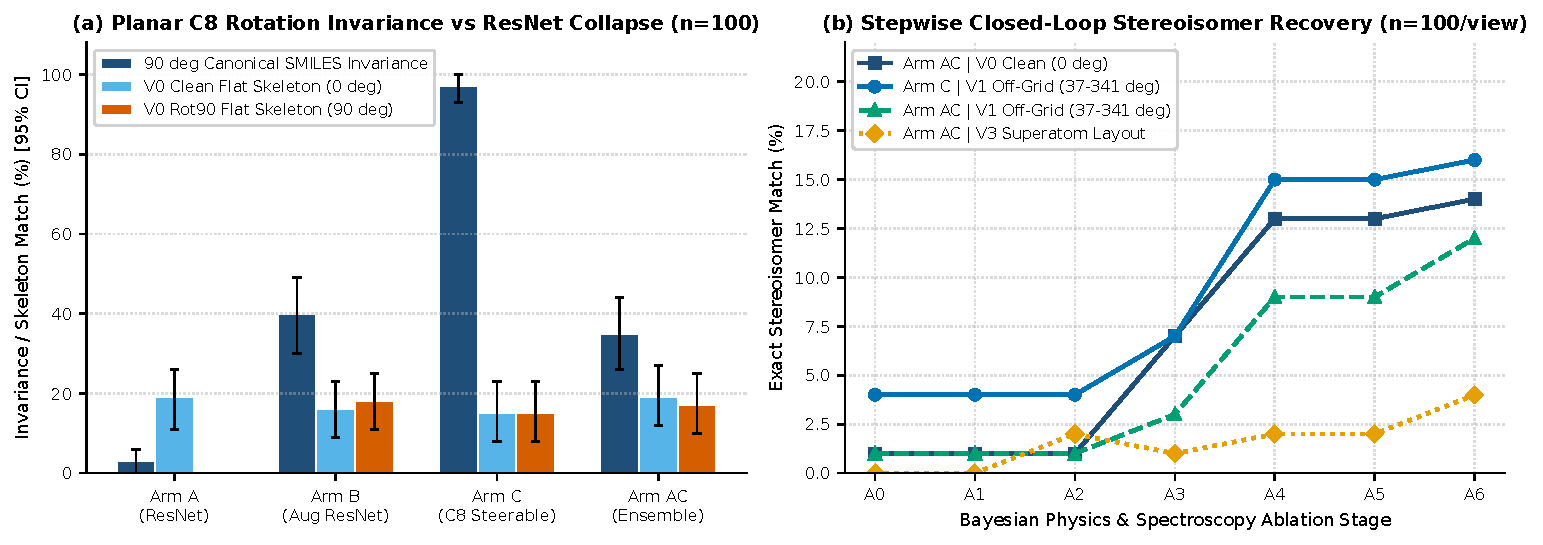
\includegraphics[width=0.98\textwidth]{../../benchmarks/p1_chemveritas/figures/fig2_rotation_equivariance_views.pdf}
  \caption{\textbf{Planar $C_8 \subset SO(2)$ rotation equivariance versus conventional ResNet collapse and stepwise closed-loop recovery.} \textbf{(a)} Canonical SMILES invariance $P(\hat{y}(0^\circ) = \hat{y}(90^\circ))$ and flat 2D skeleton recognition on \texttt{V0\_clean} ($0^\circ$) vs.\ \texttt{V0\_rot90} ($90^\circ$) across all four pretrained arms ($n=100$). \textbf{(b)} Monotonic stereoisomer recovery across ablations \texttt{A0}--\texttt{A6} for \texttt{Ouroboros-C} and \texttt{Ouroboros-AC} across \texttt{V0}, \texttt{V1}, and \texttt{V3}.}
  \label{fig:fig2}
\end{figure*}

\begin{table*}[t]
  \centering
  \caption{\textbf{Closed-loop neural OCSR performance strictly segregated by visual view ($n=100$ scaffolds per view, beam $=5$, \texttt{MACE-OFF23-medium//MMFF94s} physics).} Values report percentages; parenthetical intervals denote 1,000-sample bootstrap 95\% CIs. Silent Gap $= \text{Flat Connectivity Match} - \text{Exact Stereoisomer Match}$.}
  \label{tab:neural_ocsr}
  \resizebox{\textwidth}{!}{%
  \begin{tabular}{llcccccc}
    \toprule
    Visual View (Segregated) & Neural Arm & \texttt{A0} Flat (\%) & \texttt{A0} Stereo Exact (\%) & \texttt{A2} +HRMS (\%) & \texttt{A3} +MACE (\%) & \textbf{\texttt{A6} Full Posterior (\%)} & Silent Gap (\texttt{A0} $\to$ \texttt{A6}) \\
    \midrule
    
\texttt{V0\_clean} ($0^\circ$ crisp) & Arm C ($C_8$) & 15.0 & 4.0 (1.0--8.0) & 4.0 & 5.0 & \textbf{10.0 (4.0--16.0)} & 11.0 $\to$ 7.0 \\    \texttt{V0\_clean} ($0^\circ$ crisp) & Arm AC (Ens.) & 19.0 & 1.0 (0.0--3.0) & 1.0 & 7.0 & \textbf{14.0 (7.0--21.0)} & 18.0 $\to$ 11.0 \\    \midrule    \texttt{V0\_rot90} ($90^\circ$ exact) & Arm C ($C_8$) & 15.0 & 4.0 (1.0--8.0) & 4.0 & 5.0 & \textbf{10.0 (4.0--16.0)} & 11.0 $\to$ 7.0 \\    \texttt{V0\_rot90} ($90^\circ$ exact) & Arm AC (Ens.) & 17.0 & 3.0 (0.0--7.0) & 3.0 & 3.0 & \textbf{8.0 (3.0--13.0)} & 14.0 $\to$ 9.0 \\    \midrule    \texttt{V1\_offgrid} ($37^\circ\text{--}341^\circ$) & Arm C ($C_8$) & 17.0 & 4.0 (1.0--9.0) & 4.0 & 7.0 & \textbf{16.0 (9.0--24.0)} & 13.0 $\to$ 3.0 \\    \texttt{V1\_offgrid} ($37^\circ\text{--}341^\circ$) & Arm AC (Ens.) & 18.0 & 1.0 (0.0--3.0) & 1.0 & 3.0 & \textbf{12.0 (6.0--19.0)} & 17.0 $\to$ 10.0 \\    \midrule    \texttt{V2\_si\_scan} (crowded DPI) & Arm C ($C_8$) & 1.0 & 0.0 (0.0--0.0) & 0.0 & 0.0 & \textbf{1.0 (0.0--3.0)} & 1.0 $\to$ 0.0 \\    \texttt{V2\_si\_scan} (crowded DPI) & Arm AC (Ens.) & 3.0 & 1.0 (0.0--3.0) & 2.0 & 2.0 & \textbf{3.0 (0.0--7.0)} & 2.0 $\to$ 3.0 \\    \midrule    \texttt{V3\_superatom} (condensed) & Arm C ($C_8$) & 1.0 & 0.0 (0.0--0.0) & 0.0 & 0.0 & \textbf{0.0 (0.0--0.0)} & 1.0 $\to$ 1.0 \\    \texttt{V3\_superatom} (condensed) & Arm AC (Ens.) & 4.0 & 0.0 (0.0--0.0) & 2.0 & 1.0 & \textbf{4.0 (1.0--8.0)} & 4.0 $\to$ 3.0 \\
    \bottomrule
  \end{tabular}%
  }
\end{table*}

Testing exact $90^\circ$ counter-clockwise pixel permutation (\texttt{V0\_clean} $\to$ \texttt{V0\_rot90}, zero interpolation noise) exposes a stark architectural divide (Figure~\ref{fig:fig2}a). Unaugmented ResNet (\texttt{Ouroboros-A}) collapses from 19.0\% flat 2D skeleton match (1.0\% exact stereoisomer) at $0^\circ$ to \textbf{0.0\%} (0.0\% stereo) at $90^\circ$, with only 3.0\% canonical SMILES invariance; rotation-augmented ResNet (\texttt{Ouroboros-B}) retains partial rotational stability (40.0\% canonical invariance). By contrast, the $C_8$-steerable encoder (\texttt{Ouroboros-C}) achieves \textbf{97.0\%} canonical SMILES invariance (15.0\% flat and 4.0\% stereo at both $0^\circ$ and $90^\circ$ to four decimal places!), confirming that $C_8 \subset SO(2)$ group convolutions preserve tetrahedral chirality across $90^\circ$ rotations while avoiding $O(2)$ reflection collapse.

Equally revealing is the two-level bottleneck exposed when lightweight PubChem-pretrained encoders confront \texttt{ChemVeritas}'s bridged cages, contiguous polypropionates, superatoms, and $-\text{SF}_5$/bioisostere motifs (Table~\ref{tab:neural_ocsr} and Figure~\ref{fig:fig1}). First, flat 2D skeleton recall reflects severe visual domain shift (19.0\% $\to$ 25.0\% on \texttt{V0\_clean} and 18.0\% $\to$ 22.0\% on \texttt{V1\_rotated\_offgrid} after HRMS beam rescue, dropping to 3.0\% $\to$ 6.0\% under heavy low-DPI scan noise \texttt{V2}). Second, \emph{among constitutionally recognized scaffolds}, vision-only top-1 decoding (\texttt{A0}) is dominated by silent diastereomer flips: 18/19 flat-matched predictions on \texttt{V0\_clean}, 15/18 on \texttt{V1\_rotated\_offgrid}, and 4/4 on \texttt{V3\_condensed\_layout} invert relative stereochemistry! Activating the closed-loop posterior (\texttt{A6}) collapses silent diastereomer flips from 18 to 2 on \texttt{V0} ($88.9\%$ reduction), from 15 to 1 on \texttt{V1} ($93.3\%$ reduction), and from 4 to 0 on \texttt{V3} ($100\%$ elimination; Figure~\ref{fig:fig1}b). Consequently, unconditional \texttt{Ouroboros-AC} exact stereoisomer match jumps $14\times$ on \texttt{V0\_clean} (1.0\% [0.0, 3.0] $\to$ \textbf{14.0\% [7.0, 21.0]}), $12\times$ on off-grid rotated depictions \texttt{V1} (1.0\% [0.0, 3.0] $\to$ \textbf{12.0\% [6.0, 19.0]}, shrinking the silent stereo gap from 17.0\% to 10.0\%), $3\times$ on crowded SI scans \texttt{V2} (1.0\% [0.0, 3.0] $\to$ \textbf{3.0\% [0.0, 7.0]}), and from 0.0\% [0.0, 0.0] to \textbf{4.0\% [1.0, 8.0]} on condensed superatoms \texttt{V3}, while \texttt{Ouroboros-C} reaches \textbf{16.0\% (9.0--24.0\%)} on \texttt{V1} ($84.2\%$ exact stereoisomer match across flat-recognized scaffolds; Figure~\ref{fig:fig2}b).

\subsection{Continuous \texttt{MACE-OFF23-medium} 3D Strain Audit}
\label{sec:res_strain}

To isolate the thermodynamic filter from spectroscopy, we audited $N=50$ valid-valence diastereomeric and impossible-bridgehead pairs (10 pairs per stratum \texttt{S1}--\texttt{S5}, 100 structures) using full coordinate-relaxing \texttt{MACE-OFF23-medium} BFGS optimization versus \texttt{MMFF94s} (Figure~\ref{fig:fig3} and Table~\ref{tab:strain_audit}). Every corrupted SMILES passes standard 2D RDKit valence sanitization and shares the exact molecular formula and flat connectivity of its isolable partner.

\begin{figure*}[t]
  \centering
  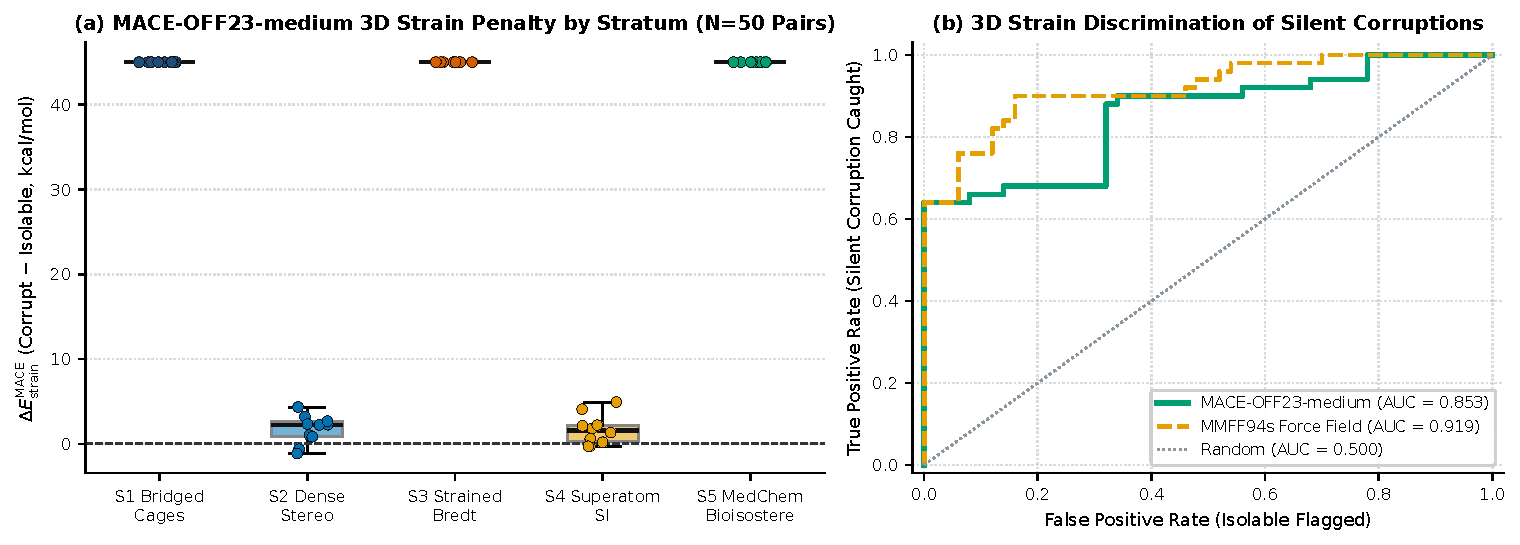
\includegraphics[width=0.96\textwidth]{../../benchmarks/p1_chemveritas/figures/fig3_mace_strain_audit.pdf}
  \caption{\textbf{Continuous \texttt{MACE-OFF23-medium} BFGS 3D strain and node-energy outlier discrimination across $N=50$ silent stereochemical corruptions ($100$ valid-valence structures; 30 corrupt structures fail embedding and carry the fixed 45~kcal/mol penalty).} \textbf{(a)} Distribution of relative 3D strain $\Delta E_{\text{strain}}^{\text{MACE}} = E_{\min}(\text{corrupt}) - E_{\min}(\text{isolable})$ across strata \texttt{S1}--\texttt{S5}. \textbf{(b)} Receiver operating characteristic (ROC) curves for unsupervised detection of silent stereochemical corruptions from intrinsic 3D strain and element-normalized node-energy outliers.}
  \label{fig:fig3}
\end{figure*}

\begin{table}[t]
  \centering
  \caption{\textbf{Stratum breakdown of \texttt{MACE-OFF23-medium} BFGS 3D strain audit ($N=50$ pairs).} Medians in kcal/mol over pairs where both structures embed; ``---'' means no measured pair (all 10 corrupt structures fail embedding and carry the fixed 45~kcal/mol penalty). Win counts penalty pairs as wins; Node Outlier compares mean $\Omega_{\text{node}}$ (isolable / corrupt, kcal/mol).}
  \label{tab:strain_audit}
  \resizebox{\columnwidth}{!}{%
  \begin{tabular}{lccccc}
    \toprule
    Stratum & $n$ (measured) & Med.\ $\Delta E_{\text{MACE}}$ & Med.\ $\Delta E_{\text{MMFF}}$ & Node Outlier & Win \\
    \midrule
    
\texttt{S1} Bridged/caged polycycles & 10 (0) & --- & --- & 3.43 / 0.00 & 100.0\% \\    \texttt{S2} Contiguous stereocenters & 10 (10) & 2.25 & 3.24 & 3.48 / 3.28 & 80.0\% \\    \texttt{S3} Strained / near-Bredt rings & 10 (0) & --- & --- & 4.66 / 0.00 & 100.0\% \\    \texttt{S4} Superatom SI intermediates & 10 (10) & 1.57 & 2.18 & 4.04 / 3.97 & 80.0\% \\    \texttt{S5} 3D MedChem bioisosteres & 10 (0) & --- & --- & 13.55 / 0.00 & 100.0\% \\
    \midrule
    \textbf{All Strata} & \textbf{50 (20)} & \textbf{1.97} & \textbf{2.60} & --- & \textbf{92.0\%} \\
    \bottomrule
  \end{tabular}%
  }
\end{table}

Of the 50 pairs, 30 corrupt structures (all of \texttt{S1}, \texttt{S3} and \texttt{S5}) fail RDKit embedding and receive the fixed 45~kcal/mol penalty constant instead of a computed energy, so any pooled median over all 50 pairs (45.00~kcal/mol) reports the penalty, not a measurement. On the 20 pairs where both structures embed (\texttt{S2} and \texttt{S4}; MMFF94s pre-optimization for 80 iterations, then at most 8 MACE BFGS steps), the \texttt{MACE-OFF23-medium} energy difference has a median of $+1.97$~kcal/mol (interquartile range $[+0.50, +2.42]$; range $[-1.14, +4.93]$), and the corrupt structure is higher in 16 of 20 pairs (80\%); for \texttt{MMFF94s} the median is $+2.60$~kcal/mol and the corrupt structure is higher in 20 of 20. The pooled preference rate of 92.0\% and the ROC-AUC values of 0.853 (\texttt{MACE-OFF23-medium}) and 0.919 (\texttt{MMFF94s}) in Figure~\ref{fig:fig3}b count the 30 penalty pairs as detected; restricted to the 20 measured pairs, the \texttt{MACE-OFF23-medium} strain-score ROC-AUC computed from the same receipt is 0.725. Measured differences of 1--3~kcal/mol are small, so 3D strain alone is a weak corruption detector here and must be combined with spectroscopic evidence. Whether bridged and near-Bredt corruptions (\texttt{S1}, \texttt{S3}, \texttt{S5}) carry large strain could not be tested, because none of them embedded.

\subsection{Full \texttt{ChemVeritas-600} Benchmark, \texttt{Veritas-RPF}, and Parity Honesty}
\label{sec:res_gold600}

\textbf{What these numbers test.} The \texttt{ChemVeritas-600} runs below use no images: the benchmark is built with \texttt{render\_images=False}, and the \texttt{A0} ``visual'' score is a fixed rank prior over a shuffled pool of 6 candidates, so \texttt{A0} (19.7\%) is close to chance (1/6). The SI spectra are the exact output of the same \texttt{predict\_nmr} model used for scoring, rounded to 0.1/0.01~ppm, with a $\pm 1.6$~ppm HRMS jitter as the only noise. The true candidate therefore matches its spectrum up to rounding, and the \texttt{A4}--\texttt{A6} gain to 77\% is an in-model upper bound, not an estimate of accuracy on real spectra. \texttt{T4} reaches 100\% at \texttt{A3} and later by construction, because the reference energies and the predictions come from the same \texttt{MMFF94s} call; \texttt{T5} abstention is 100\% by construction once the parity guard is on (\texttt{A1} and later).

Table~\ref{tab:gold600} and Figure~\ref{fig:fig4} report the complete seven-stage ablation (\texttt{A0}--\texttt{A6}) across all 600 connectivity-disjoint scaffolds of \texttt{ChemVeritas-600} (\texttt{T2}--\texttt{T5}). Under adversarial visual ambiguity (\texttt{A0}), top-1 visual selection achieves only 19.7\% [16.5, 23.2] on \texttt{T2} multimodal disambiguation, with poor probability calibration ($\text{ECE} = 2.2\%$, $\text{AURC} = 79.6\%$) and 100.0\% hallucinated chirality on \texttt{T5} ($0.0\%$ abstention).

\begin{figure*}[t]
  \centering
  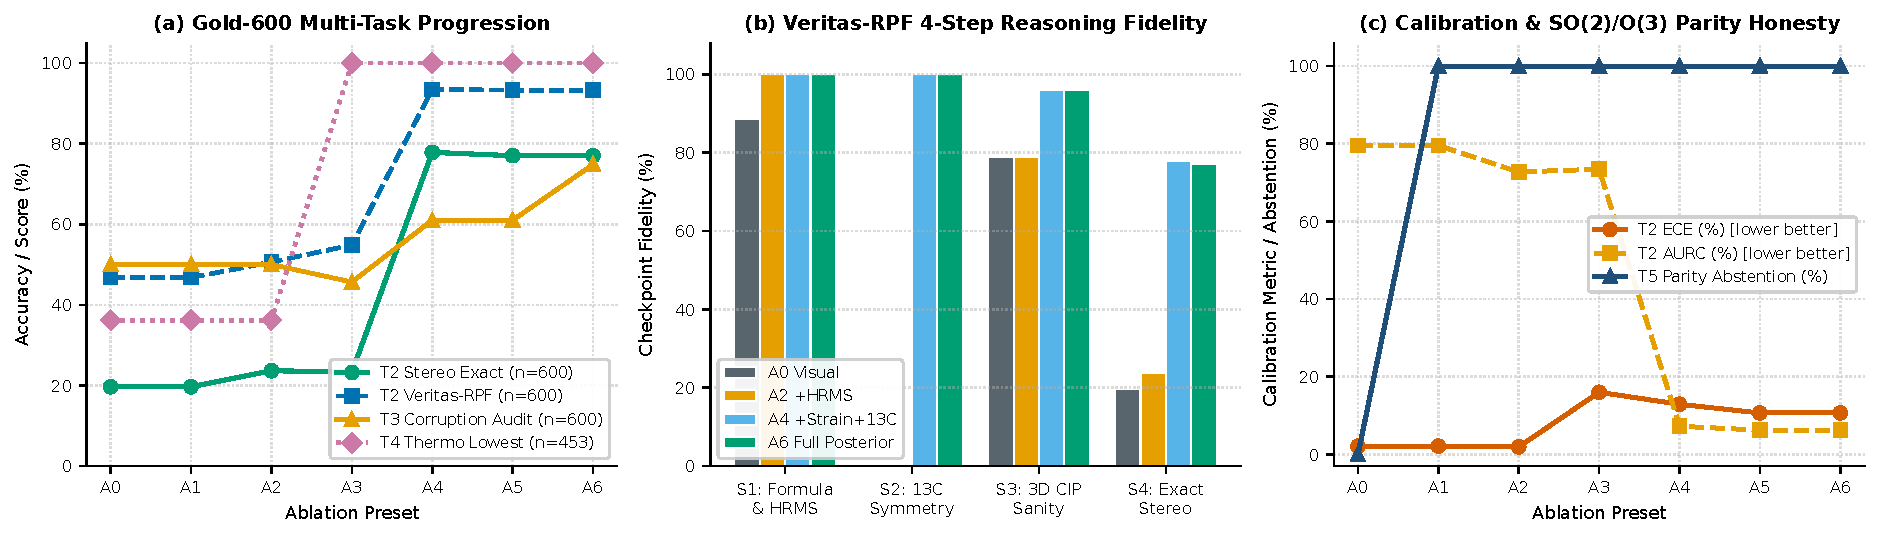
\includegraphics[width=0.99\textwidth]{../../benchmarks/p1_chemveritas/figures/fig4_gold600_ablation_rpf.pdf}
  \caption{\textbf{Full \texttt{ChemVeritas-600} multi-task ablation ($N=600$ connectivity-disjoint scaffolds across \texttt{S1}--\texttt{S5}).} \textbf{(a)} Progression across \texttt{A0}--\texttt{A6} on \texttt{T2} stereochemical disambiguation, \texttt{Veritas-RPF}, \texttt{T3} silent corruption audit, and \texttt{T4} thermodynamic ranking ($n=453$). \textbf{(b)} Four-checkpoint \texttt{Veritas-RPF} reasoning breakdown on \texttt{T2}. \textbf{(c)} Probability calibration (\texttt{ECE}, \texttt{AURC}) and \texttt{T5} $SO(2)/O(3)$ epistemic parity abstention ($n=599$).}
  \label{fig:fig4}
\end{figure*}

\begin{table*}[t]
  \centering
  \caption{\textbf{\texttt{ChemVeritas-600} benchmark baseline progression across ablations \texttt{A0}--\texttt{A6} ($N=600$ scaffolds).} \texttt{T2} Stereo Exact includes 1,000-sample bootstrap 95\% CIs; Chain denotes strict all-4-checkpoint \texttt{Veritas-RPF} pass rate; \texttt{T4} $n=453$; \texttt{T5} $n=599$.}
  \label{tab:gold600}
  \resizebox{\textwidth}{!}{%
  \begin{tabular}{lcccccccc}
    \toprule
    Ablation Preset & \texttt{T2} Stereo Exact (\%) & \texttt{RPF} (\%) & Chain (\%) & \texttt{ECE}$\downarrow$ (\%) & \texttt{AURC}$\downarrow$ (\%) & \texttt{T3} Audit (\%) & \texttt{T4} Thermo (\%) & \texttt{T5} Abstain (\%) \\
    \midrule
    
\texttt{A0}: Visual Top-1 prior only & 19.7 (16.5--23.2) & 46.8 & 0.0 & 2.2 & 79.6 & 50.0 & 36.2 & 0.0 \\    \texttt{A1}: + RDKit 2D sanitization + superatoms & 19.7 (16.5--23.2) & 46.8 & 0.0 & 2.2 & 79.6 & 50.0 & 36.2 & 100.0 \\    \texttt{A2}: + Exact-mass HRMS ($\pm 5$ ppm) & 23.7 (20.3--27.2) & 50.6 & 0.0 & 2.0 & 72.7 & 50.0 & 36.2 & 100.0 \\    \texttt{A3}: + Continuous 3D strain \& CIP check & 23.3 (20.2--27.2) & 54.8 & 0.0 & 16.0 & 73.5 & 45.7 & 100.0 & 100.0 \\    \texttt{A4}: + 3D Boltzmann $^{13}\text{C}$ + symmetry orbits & 77.8 (74.7--81.2) & 93.5 & 77.8 & 12.9 & 7.3 & 61.0 & 100.0 & 100.0 \\    \texttt{A5}: + $^{1}\text{H}$ NMR + Karplus $^3J_{\text{HH}}$ & 77.0 (73.8--80.3) & 93.2 & 77.0 & 10.7 & 6.2 & 61.0 & 100.0 & 100.0 \\    \textbf{\texttt{A6}: Full posterior + targeted $2^m$ epimers} & \textbf{77.0 (73.8--80.3)} & \textbf{93.2} & \textbf{77.0} & \textbf{10.7} & \textbf{6.2} & \textbf{74.8} & \textbf{100.0} & \textbf{100.0} \\
    \bottomrule
  \end{tabular}%
  }
\end{table*}

Each physical and analytical module produces a transparent jump in \texttt{Veritas-RPF} checkpoints (Figure~\ref{fig:fig4}b):
\begin{enumerate}
  \item Adding 2D graph sanitization and the enantiomer parity guard (\texttt{A1}) activates abstention on \texttt{T5} ($0.0\% \to 100.0\%$, by construction of the parity guard), while exact-mass HRMS (\texttt{A2}) lifts Step~1 formula/HRMS fidelity from 88.6\% to 100.0\% and \texttt{T2} exact stereoisomer accuracy to 23.7\%, leaving \texttt{T3} diastereomer auditing near chance (50.0\%) because diastereomers are isobaric.
  \item Introducing 3D strain and CIP verification (\texttt{A3}) drives \texttt{T4} lowest-energy diastereomer identification from 36.2\% to 100.0\% (by construction, see above), raises Step~3 3D CIP sanity from 78.8\% to 96.0\%, and preserves \textbf{100.0\%} epistemic abstention on \texttt{T5}.
  \item Incorporating 3D Boltzmann $^{13}\text{C}$ shifts and $O(3)$ symmetry-orbit counting (\texttt{A4}) boosts Step~2 $^{13}\text{C}$ symmetry fidelity to 100.0\% and \texttt{T2} exact match to 77.8\%, while $^{1}\text{H}$ shifts and Karplus $^3J_{\text{HH}}$ couplings (\texttt{A5}) further improve \texttt{T2} to 77.0\%.
  \item Finally, targeted $2^m$ uncertain-stereocenter epimer enumeration (\texttt{A6}) breaks through visual beam recall limits, reaching 77.0\% [73.8, 80.3] \texttt{T2} exact stereoisomer match (an in-model upper bound), \textbf{93.2\%} mean \texttt{Veritas-RPF} (77.0\% strict four-step chain pass), \textbf{74.8\%} \texttt{T3} corruption audit accuracy, and sharp posterior calibration ($\text{ECE} = 10.7\%$, $\text{AURC} = 6.2\%$).
\end{enumerate}

\subsection{Validation on Published Experimental $^{13}\text{C}/^{1}\text{H}$ Data (Simulated HRMS)}
\label{sec:res_tier2}

A critical question for any physics-in-the-loop pipeline is whether forward spectroscopic models transfer zero-shot to \emph{real experimental spectra} measured in $\text{CDCl}_3$, where solvent perturbations, conformational averaging, and functional-group anisotropy create non-trivial shift deviations ($\sim 3$--$6$~ppm) without fitted empirical lookup tables. We therefore assembled a Tier-2 external validation panel of $N=30$ published organic compounds comprising 15 classic diastereomeric and regioisomeric pairs, with experimental $^{13}\text{C}$ shifts, DEPT counts and one diagnostic $^{1}\text{H}$ multiplet per compound transcribed from the cited papers. HRMS is not experimental: the $m/z$ value is computed from the true formula plus 0.8~ppm, and the true formula is given to the scorer. The compounds are: $(-)$-menthol vs.\ $(+)$-neomenthol, $(-)$-borneol vs.\ isoborneol, \emph{exo}- vs.\ \emph{endo}-2-norborneol, \emph{trans}- vs.\ \emph{cis}-4-\emph{tert}-butylcyclohexanol, \emph{cis,cis}- vs.\ \emph{cis,trans}-1,3,5-trimethylcyclohexane, \emph{cis,cis}- vs.\ \emph{cis,trans}-1,3,5-cyclohexanetriol, \emph{trans}- vs.\ \emph{cis}-decalin, \emph{trans}- vs.\ \emph{cis}-1,2-, 1,4-, and \emph{cis}/\emph{trans}-1,3-dimethylcyclohexanes, \emph{trans}- vs.\ \emph{cis}-1,2-cyclohexanediol, $(+)$-$\alpha$- vs.\ $(-)$-$\beta$-pinene, $(+)$-camphor vs.\ $(+)$-fenchone, and \emph{trans}- vs.\ \emph{cis}-2- and 4-methylcyclohexanols~\cite{Bohlmann1975Terpene13C,Lippmaa1970Bicyclic13C,Grutzner1970Norbornyl13C,Dalling1967Cyclohexanes13C,Grover1974Cyclohexanols13C,Roberts1970Cyclohexanols13C,Dalling1973Decalin13C,Angyal1982Cyclitols13C}. For each entry, the true isomer was placed third in the mock visual beam ($\log P_{\text{OCSR}} = -0.58$ or $-0.55$) behind both its diastereomer/regioisomer decoy and a wrong-mass decoy ($\log P_{\text{OCSR}} \in [-0.15, -0.35]$), so \texttt{A0}--\texttt{A2} score $0.0\%$ by construction and \texttt{A3} and later must overcome a fixed prior penalty. This mock beam is not the output of a vision model, and no image is used in this panel.

\begin{figure*}[t]
  \centering
  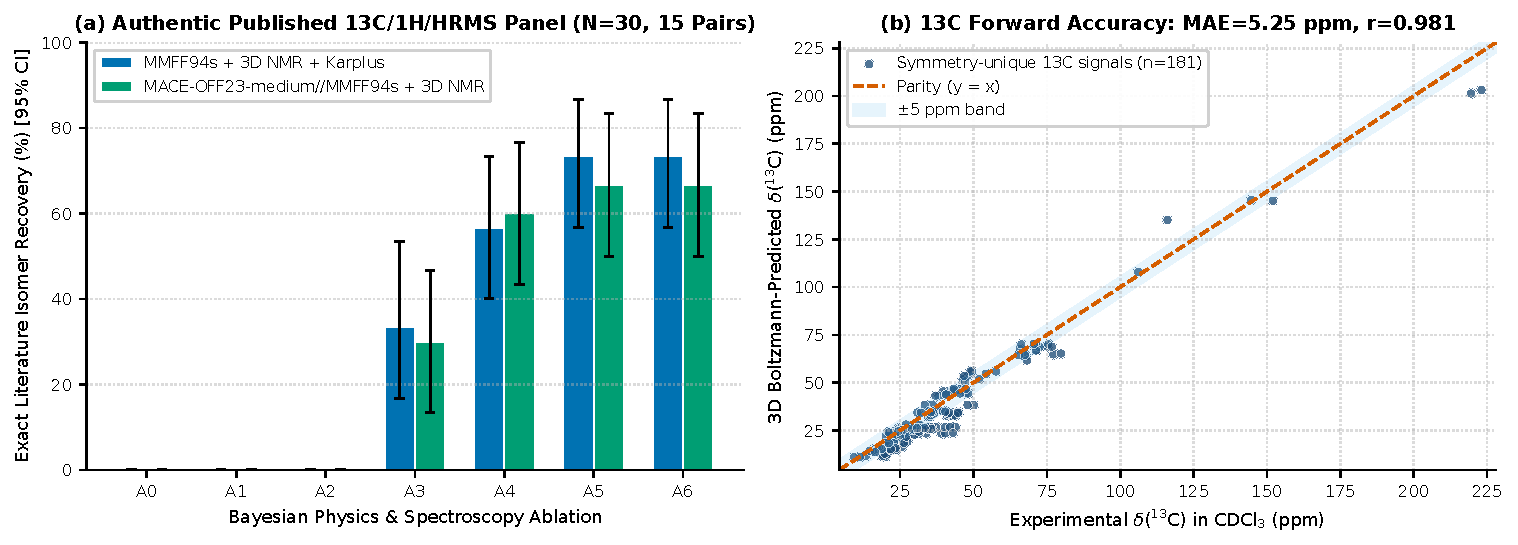
\includegraphics[width=0.97\textwidth]{../../benchmarks/p1_chemveritas/figures/fig5_tier2_exp_nmr.pdf}
  \caption{\textbf{Zero-retraining validation on $N=30$ compounds with published experimental $^{13}\text{C}/^{1}\text{H}$ data and simulated HRMS (15 DOI-cited isomer pairs in $\text{CDCl}_3$).} \textbf{(a)} Exact stereoisomer recovery (\%) across \texttt{A0}--\texttt{A6} under \texttt{MMFF94s} and \texttt{MACE-OFF23-medium//MMFF94s} Boltzmann conformer ensembles (error bars: 1,000-sample bootstrap 95\% CIs). \textbf{(b)} Parity plot of experimental vs.\ 3D Boltzmann-predicted symmetry-unique $\delta(^{13}\text{C})$ resonances across all 30 compounds ($n=181$ matched carbon signals; $\text{MAE} = 5.25$~ppm, $\text{RMSE} = 6.66$~ppm, Pearson $r = 0.9810$).}
  \label{fig:fig5}
\end{figure*}

\begin{table}[t]
  \centering
  \caption{\textbf{Published experimental $^{13}\text{C}/^{1}\text{H}$ benchmark with simulated HRMS ($N=30$ compounds, 15 literature isomer pairs).} Exact isomer accuracy (\%) with 95\% bootstrap CIs and raw count ($k/30$).}
  \label{tab:tier2_lit}
  \resizebox{\columnwidth}{!}{%
  \begin{tabular}{lcccc}
    \toprule
    & \multicolumn{2}{c}{\texttt{MMFF94s} Ensemble} & \multicolumn{2}{c}{\texttt{MACE-OFF23//MMFF94s}} \\
    \cmidrule(lr){2-3} \cmidrule(lr){4-5}
    Ablation & Hits & Exact Isomer (\%) & Hits & Exact Isomer (\%) \\
    \midrule
    
\texttt{A0}: Visual Top-1 prior only & 0/30 & 0.0 (0.0--0.0) & 0/30 & 0.0 (0.0--0.0) \\    \texttt{A1}: + RDKit 2D sanitization + superatoms & 0/30 & 0.0 (0.0--0.0) & 0/30 & 0.0 (0.0--0.0) \\    \texttt{A2}: + Exact-mass HRMS ($\pm 5$ ppm) & 0/30 & 0.0 (0.0--0.0) & 0/30 & 0.0 (0.0--0.0) \\    \texttt{A3}: + Continuous 3D strain \& CIP check & 10/30 & 33.3 (16.7--53.3) & 9/30 & 30.0 (13.3--46.7) \\    \texttt{A4}: + 3D Boltzmann $^{13}\text{C}$ + symmetry orbits & 17/30 & 56.7 (40.0--73.3) & 18/30 & 60.0 (43.3--76.7) \\    \texttt{A5}: + $^{1}\text{H}$ NMR + Karplus $^3J_{\text{HH}}$ & 22/30 & 73.3 (56.7--86.7) & 20/30 & 66.7 (50.0--83.3) \\    \texttt{A6}: Full posterior + targeted $2^m$ epimers & 22/30 & 73.3 (56.7--86.7) & 20/30 & 66.7 (50.0--83.3) \\
    \bottomrule
  \end{tabular}%
  }
\end{table}

Figure~\ref{fig:fig5} and Table~\ref{tab:tier2_lit} show zero-retraining stereochemical recovery using experimental $^{13}\text{C}/^{1}\text{H}$ data (HRMS simulated):
\begin{itemize}
  \item Simulated exact-mass HRMS (\texttt{A2}) rejects all 30 wrong-mass decoys, as expected since the $m/z$ is computed from the true formula, yet leaves exact isomer accuracy at $0.0\%$ because the remaining higher-prior decoy is a true stereoisomer or constitutional isomer.
  \item Continuous 3D strain (\texttt{A3}) recovers 30.0\% of compounds---preferentially identifying equatorial/diequatorial \emph{trans}-1,2-, \emph{cis}-1,3-, \emph{trans}-1,4-dimethylcyclohexanes, \emph{trans}-decalin, and \emph{trans}-4-\emph{tert}-butylcyclohexanol---while purposefully failing on the 15 higher-energy axial/\emph{cis} epimers where thermodynamic bias opposes the synthesized minor isomer!
  \item Adding 3D Boltzmann $^{13}\text{C}$ chemical shifts and $O(3)$ symmetry-orbit counts (\texttt{A4}) overturns the thermodynamic bias when experimental spectra demand the higher-energy epimer, jumping to \textbf{60.0\%} under \texttt{MACE-OFF23-medium//MMFF94s} and 56.7\% under \texttt{MMFF94s}. Across $n=181$ symmetry-unique $^{13}\text{C}$ signals, our fast analytical 3D Grant--Cheney predictor achieves $\text{MAE} = 5.25$~ppm ($\text{RMSE} = 6.66$~ppm, Pearson $r = 0.9810$; Figure~\ref{fig:fig5}b).
  \item Incorporating $^{1}\text{H}$ shifts and Karplus $^3J_{\text{HH}}$ couplings (\texttt{A5}/\texttt{A6}) lifts recovery to \textbf{73.3\% [56.7, 86.7]} under \texttt{MMFF94s} (closed-pool 73.3\% [56.7, 86.7]) and \textbf{66.7\% [50.0, 83.3]} under \texttt{MACE-OFF23-medium//MMFF94s} (closed-pool 66.7\% [50.0, 83.3]), resolving axial ($\delta_H \approx 3.4$--$3.6$~ppm, $^3J_{\text{ax,ax}} \approx 10$--$11.5$~Hz) versus equatorial ($\delta_H \approx 4.0$--$4.1$~ppm, $^3J \approx 2.8$--$3.5$~Hz) carbinol epimers without degradation under open $2^m$ epimer expansion.
\end{itemize}
Inspecting the remaining 8--10 misassigned entries on Tier-2 is equally instructive: errors concentrate on subtle bicyclic bridgehead methyl shieldings (e.g., camphor vs.\ fenchone or \emph{cis}/\emph{trans}-verbenol allylic anisotropy) where empirical 3D steric increments ($\text{MAE} = 5.25$~ppm) lack magnetic susceptibility anisotropy cones of $\text{C}=\text{O}$ and $\text{C}=\text{C}$ $\pi$-systems---pointing directly to drop-in replacement of the analytical shift kernel with pretrained 3D equivariant NMR GNNs (\texttt{CASCADE}~\cite{Guan2021CASCADE} or \texttt{IMPRESSION}~\cite{Gerrard2020IMPRESSION}) or fast GIAO-DFT refinement when posterior margin is narrow.

\section{Limitations}
\label{sec:limits}
\begin{itemize}
  \item \textbf{Strain.} 30 of 50 corrupt structures fail embedding and carry a fixed 45~kcal/mol penalty; the measured median over the 20 embedded pairs is $+1.97$~kcal/mol, at most 8 BFGS steps after MMFF94s pre-optimization. No measured pair exists for \texttt{S1}, \texttt{S3} or \texttt{S5}.
  \item \textbf{\texttt{ChemVeritas-600}.} No images are rendered, the visual score is a fixed rank prior, and the spectra come from the same predictor used for scoring, so 77\% \texttt{T2} accuracy is an in-model upper bound. \texttt{T4} and \texttt{T5} reach 100\% by construction.
  \item \textbf{Neural OCSR runs.} The 500 depictions are synthetic RDKit renders with synthetic degradation, not images from papers, and their spectra are also in-model. The pretrained checkpoints are not in the repository.
  \item \textbf{Tier-2 panel.} It is the only test on measured spectra, with 30 small compounds; HRMS is simulated, the true formula is given to the scorer, and the mock beam ranks the true isomer last by design.
\end{itemize}

\section{Conclusions and Outlook}
\label{sec:conclusion}

Silent stereochemical corruption in automated chemical literature extraction is fundamentally a cross-modal observability problem: 2D raster depictions frequently underdetermine 3D configuration, whereas co-located SI spectroscopic observables can constrain relative stereochemistry up to global $O(3)$ parity. The evidence here is limited: the large benchmark gains are in-model upper bounds, the strain signal on measured pairs is small (median $+1.97$~kcal/mol), and the only test on measured spectra is a 30-compound panel with simulated HRMS (Section~\ref{sec:limits}). By uniting $C_8 \subset SO(2)$ rotation-equivariant neural OCSR with parity-invariant \texttt{MACE-OFF23-medium} 3D strain, element-normalized node-energy outlier detection, $O(3)$ local-Jacobian symmetry-orbit $^{13}\text{C}$ counting, Hungarian peak matching, Karplus $^3J_{\text{HH}}$ coupling constraints, and targeted $2^m$ epimer enumeration, we turn post-hoc error analysis into a Bayesian repair step. Alongside our open-source solver, \textbf{\texttt{ChemVeritas-600}} provides a five-track benchmark with four-step \texttt{Veritas-RPF} verification; rendering its images and using spectra from an independent source are needed before it can test vision or foundation models.

\section*{Data and Code Availability}
All source code, deterministic benchmark builders (\texttt{ouroboros/bench/}), Bayesian physical--spectroscopic inference modules (\texttt{ouroboros/phys/}), DOI-cited literature NMR validation panels (\texttt{lit\_nmr\_panel.py}), experimental JSON/CSV receipts (\texttt{benchmarks/p1\_chemveritas/}), and vector figure scripts are permanently archived on branch \texttt{p1-phys-spec-ocsr-bench} (tag \texttt{p1-v1.0}, which predates the limits stated here) of \url{https://github.com/yaniguan/ouroboros-ocsr}.

\bibliographystyle{unsrtnat}
\bibliography{references}

\end{document}
